\documentclass[final]{nesy2026}

 % The following packages will be automatically loaded:
 % amsmath, amssymb, natbib, graphicx, url, algorithm2e

 %\usepackage{rotating}% for sideways figures and tables
\usepackage{longtable}% for long tables

 % The booktabs package is used by this sample document
 % (it provides \toprule, \midrule and \bottomrule).
 % Remove the next line if you don't require it.
\usepackage{booktabs}

\usepackage[T1]{fontenc}
\usepackage[utf8]{inputenc}
\usepackage{array}

 % Use \Name{Author Name} to specify the name.

 % Spaces are used to separate forenames from the surname so that
 % the surnames can be picked up for the page header and copyright footer.

 % If the surname contains spaces, enclose the surname
 % in braces, e.g. \Name{John {Smith Jones}} similarly
 % if the name has a "von" part, e.g \Name{Jane {de Winter}}.
 % If the first letter in the forenames is a diacritic
 % enclose the diacritic in braces, e.g. \Name{{\'E}louise Smith}

 % *** Make sure there's no spurious space before \nametag ***

\title[Dynamic Evidential Routing]{Dynamic Evidential Routing: A Neurosymbolic Transformer Interface for Auditable Clinical Prediction Under Extreme Missingness}

 % Two authors with the same address
\clearauthor{\Name{Arjun Vijay Prakash} \Email{arjunv.prakash12345@gmail.com}\\
\addr City Montessori School, Lucknow, Uttar Pradesh, India}

\begin{document}

\maketitle

\begin{abstract}
Dynamic evidential routing adds an auditable expert-intervention channel to transformer inference while preserving comparable held-out predictive behavior. The interface maps Monte Carlo dropout uncertainty into Non-Axiomatic Logic (NAL) truth values, revises those values with explicit clinical rules, and uses revised confidence to gate attention. Every intervention exports its trigger, neural and symbolic truth values, revision, and attention effect. We evaluate TCGA-THCA lymph node metastasis prediction as a clinical-genomic feasibility check and WiDS ICU hospital-mortality prediction as the primary high-missingness scale test. The symbolic path is active at scale, firing 13,031 times across 8,551 of 13,757 held-out ICU stays. On WiDS, paired Brier and ECE differences favor NARS-gated routing over the ungated transformer, but comparisons with flat-confidence and MC-confidence-only gating include zero. The results therefore support confidence-gated, auditable intervention without isolating symbolic revision as the cause of the calibration difference. The implementation is a NAL truth-value interface, not a full Non-Axiomatic Reasoning System (NARS) cognitive architecture or a clinically validated decision device.
\end{abstract}

\section{Introduction}
\label{sec:intro}

Clinical AI systems need more than discrimination: reviewers must be able to inspect weak evidence and expert interventions. A sparse ICU record may contain a few abnormal measurements, many unmeasured variables, and an apparently precise risk score. Missingness, irregular measurement, and cohort shift are common in hospital data, yet standard neural predictors usually collapse the available evidence into one probability \citep{ma2019,ovadia2019,ghassemi2021}. An overconfident error is then difficult to defer, audit, or correct.

The challenge is that current model components expose different pieces of the problem but do not connect them cleanly. Transformers are flexible function approximators for clinical prediction \citep{rasmy2021,azizi2021,li2019}, but attention weights are not themselves evidential confidences. Uncertainty estimators can summarize prediction instability, but they usually do not provide a symbolic intervention point. Rule-based explanations can be readable, but post-hoc rules often describe a prediction without changing the computation. What is missing is an inference-time interface in which neural uncertainty, symbolic evidence, and attention control share an auditable representation.

We propose dynamic evidential routing as that interface. A neural predictive distribution is first mapped into a two-dimensional truth value $(f,c)$, where frequency $f$ describes the balance of evidence and confidence $c$ describes evidential support \citep{wang1995,wang2006,wang2013}. Explicit clinical rules then revise feature-level truths in the same NAL truth-value space, and the revised confidence values control a normalized attention gate. This design separates what the model predicts from how strongly the available evidence supports that prediction.

We evaluate the interface on two complementary clinical benchmarks. TCGA-THCA tests the mechanism under clinical-genomic feature fusion; WiDS ICU hospital-mortality prediction tests scale and extreme missingness. The contribution is an operational neurosymbolic intervention path with arithmetic traces, quantitative coverage and fidelity checks, and comparable held-out predictive behavior. The controls also delimit the claim: they do not isolate symbolic revision as a source of improved calibration.

Figure~\ref{fig:pipeline} summarizes the inference-time data flow from sparse clinical inputs through uncertainty estimation, NAL-style truth initialization, rule-triggered revision, confidence-gated attention, and trace export.

\begin{figure}[t]
\centering
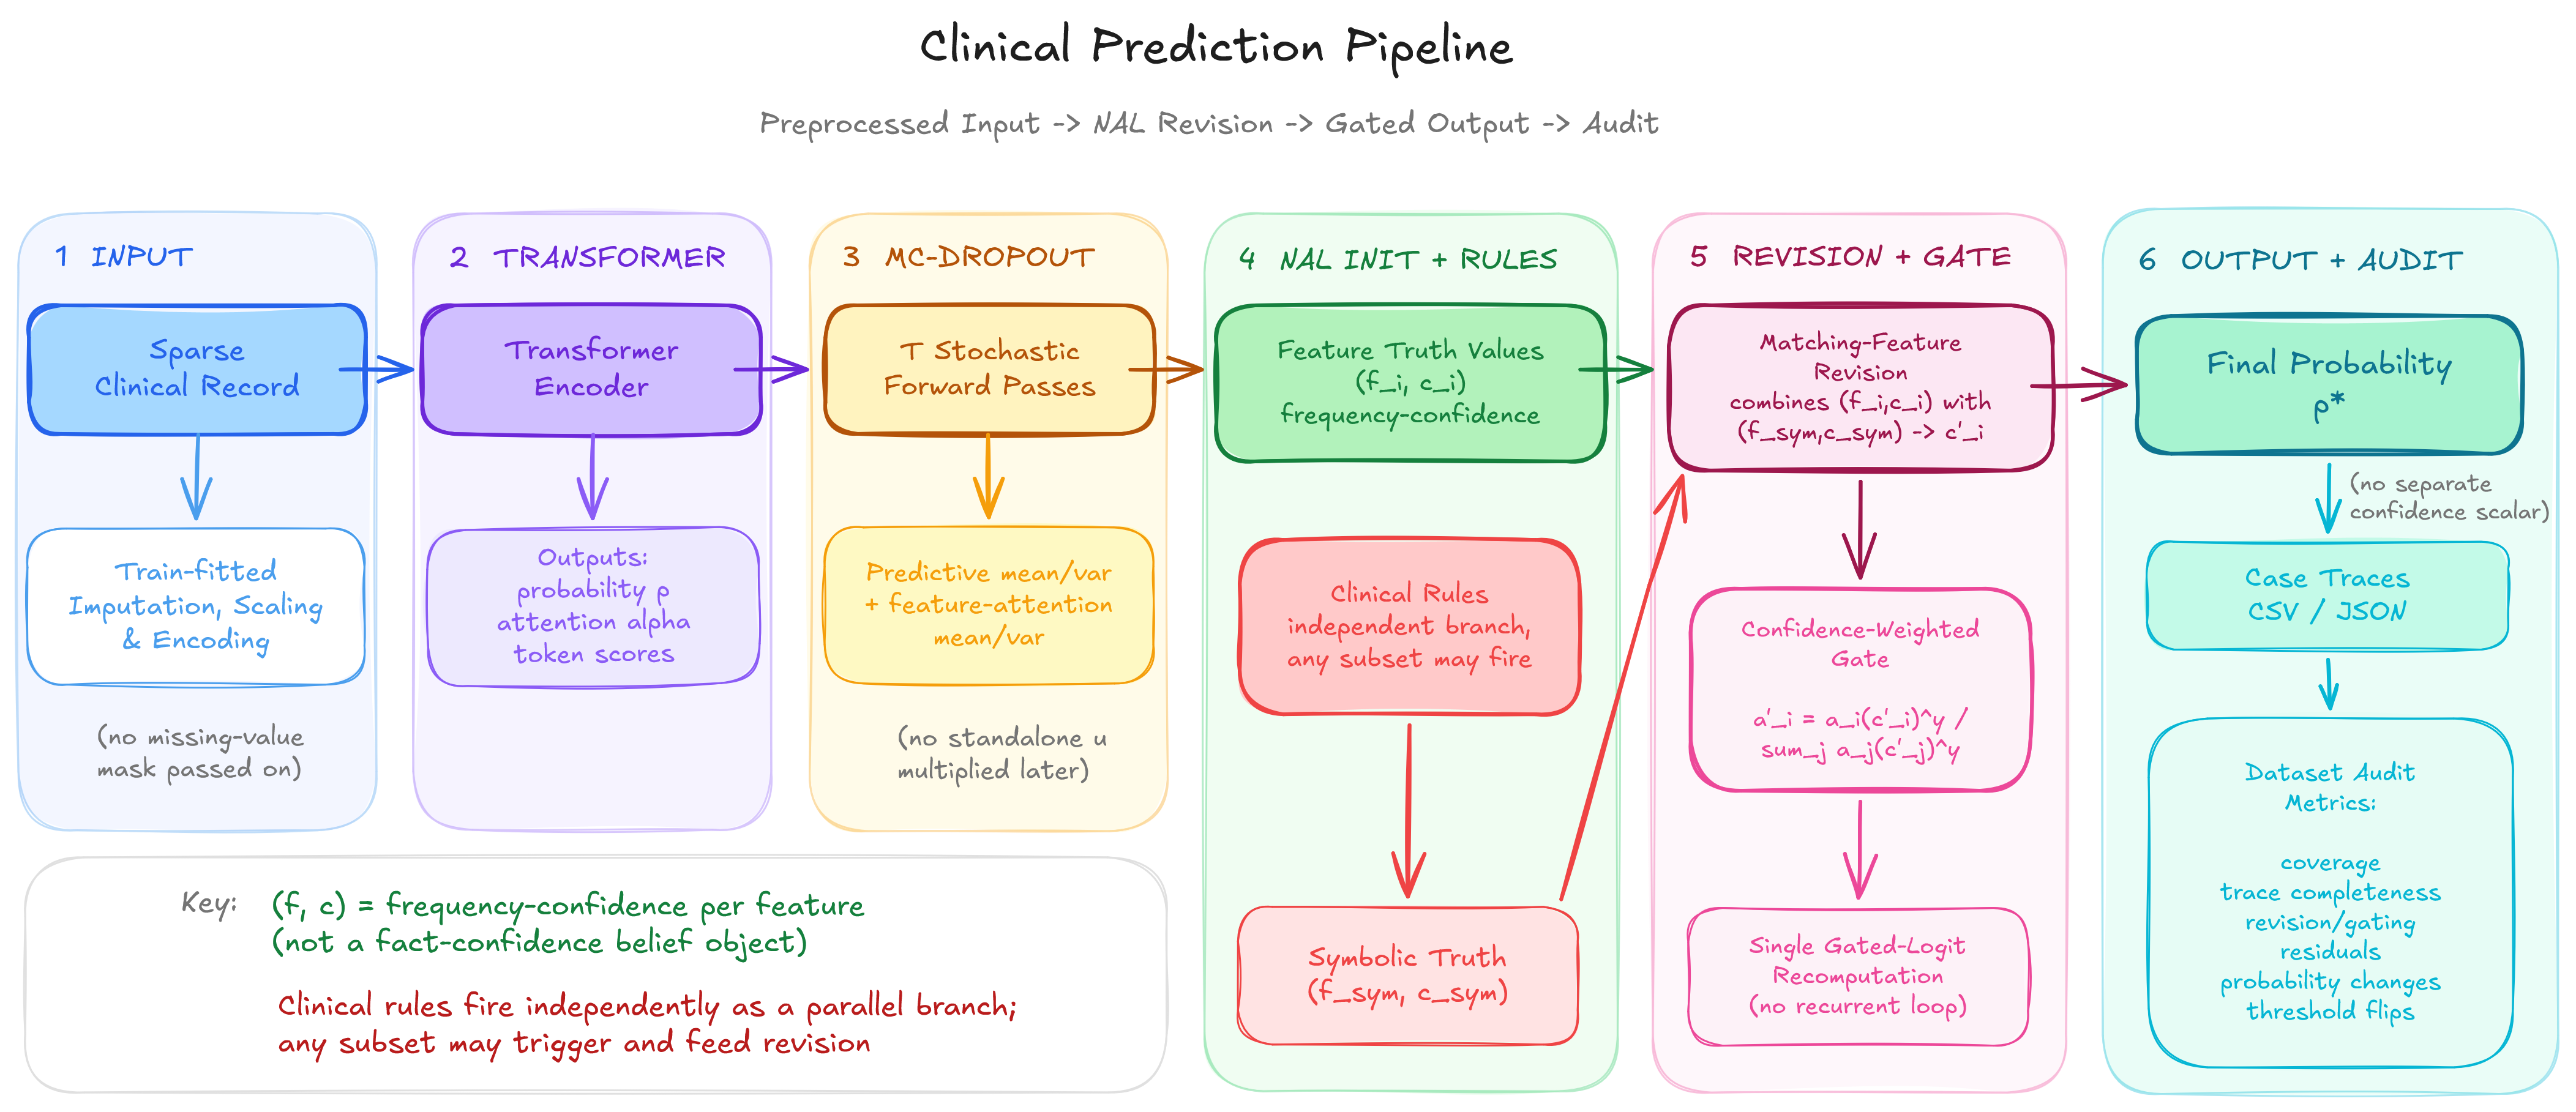
\includegraphics[width=\linewidth]{figures/figure-1.png}
\caption{Inference-time dynamic evidential routing. A trained transformer produces a prediction and feature attention; MC dropout estimates uncertainty; the uncertainty signal initializes NAL truth values; triggered clinical rules revise those values; revised confidence gates attention; and the system exports a case-level trace showing where symbolic evidence changed the computation.}
\label{fig:pipeline}
\end{figure}

\section{Related Work}
\label{sec:related}

\paragraph{Neurosymbolic integration.}
Neurosymbolic AI combines neural pattern recognition with symbolic reasoning, knowledge injection, or interpretable rule systems \citep{garcez2020,marra2021,bhuyan2024,colelough2025}. Prior surveys distinguish loose coupling, tight coupling, and unified architectures \citep{hilario2013,nawaz2025}. Dynamic evidential routing is a tight inference-time interface: the neural model supplies probabilities, uncertainty estimates, and attention weights, while the symbolic layer revises evidential confidence before attention is updated. Its contribution is the interface contract between these components. Neural uncertainty is converted into an explicit truth-value representation, symbolic rules revise that representation, and the revised confidence is fed back into attention with a trace of the intervention.

\paragraph{Clinical transformers and uncertainty.}
Clinical transformers have been used for structured EHRs, clinical text, and medical prediction tasks \citep{rasmy2021,li2019,dai2025}. Attention can help interpretability, but medical attention mechanisms rarely represent uncertainty as a first-class control signal \citep{goncalves2022}. In parallel, uncertainty quantification methods such as Bayesian neural networks, MC dropout, and ensembles provide useful but imperfect epistemic uncertainty estimates \citep{blundell2015,gal2016,lakshminarayanan2017,abad2025}. MC dropout is attractive because it is cheap, but it can be miscalibrated under dataset shift \citep{ovadia2019}. Our use of uncertainty is therefore not a standalone calibration method. The uncertainty estimate initializes evidential confidence, which becomes available for symbolic revision and case-level audit.

\paragraph{NARS and biomedical reasoning.}
NARS and Non-Axiomatic Logic model reasoning under insufficient knowledge and resources \citep{wang1995,wang2006,wang2022}. NAL truth values have been studied for uncertain medical diagnosis \citep{wang2013}. Biomedical knowledge graphs and symbolic reasoning can improve clinical interpretability \citep{wu2023,abusalih2023,rajabi2022,jiang2024,chudasama2025}, but many such systems enrich representations rather than exposing an evidential confidence variable that directly controls neural inference. This paper uses NAL truth-value functions and rule-triggered revision only. It does not implement full NARS concept memory, task scheduling, resource allocation, or evidential-base management.

The closest families differ at the intervention boundary. Ordinary attention gating has no separately inspectable symbolic judgment; uncertainty calibration changes confidence without a rule-level intervention trace; post-hoc rules describe a completed decision; and training-time knowledge injection generally requires retraining to change the symbolic source. Dynamic evidential routing instead gives uncertainty and rules a shared truth-value interface, lets rules change inference in one pass, and preserves the source and arithmetic of that change. It does not claim a new general logic or a complete NARS architecture.

\section{Method}
\label{sec:method}

\subsection{Interface Boundary}

The implementation should be read as a NAL truth-value interface inspired by NARS, not as a full NARS system. It uses the $(f,c)$ truth-value representation, deduction-style grounding of triggered rules, and revision of neural and symbolic judgments. It does not maintain concept memory, task queues, priority dynamics, resource-bounded control, or explicit evidential-base objects. The claims in this paper are therefore interface-level claims about truth-value-guided fusion and attention control.

\subsection{Truth Values}

For a statement $S$ with positive evidence $w^+$ and negative evidence $w^-$, NAL represents truth as $(f,c)$:
\begin{equation}
f=\frac{w^+}{w^+ + w^-},
\label{eq:frequency}
\end{equation}
\begin{equation}
c=\frac{w^+ + w^-}{w^+ + w^- + k}.
\label{eq:confidence}
\end{equation}
We use the standard default $k=1$, so $c=W/(W+1)$ for total evidence $W=w^+ + w^-$. Strong deduction combines two premises by
\begin{equation}
f=f_1f_2,\qquad c=f_1c_1f_2c_2.
\label{eq:deduction}
\end{equation}
Revision merges two judgments with weights $\omega_i=c_i/(1-c_i)$:
\begin{equation}
f=\frac{\omega_1 f_1+\omega_2 f_2}{\omega_1+\omega_2},\qquad
c=\frac{\omega_1+\omega_2}{\omega_1+\omega_2+1}.
\label{eq:revision}
\end{equation}
Standard NAL revision assumes disjoint evidential bases \citep{wang2024draft}. The implementation treats neural and symbolic sources as distinct when revision is invoked, but it does not store evidential bases as runtime objects.

\subsection{Neural-to-Symbolic Initialization}

For a neural probability $p$ and MC-dropout predictive variance $\sigma^2$, the initial truth value is
\begin{equation}
f_{\text{neural}}=p,\qquad
c_{\text{neural}}=\frac{p(1-p)}{p(1-p)+\sigma^2+\varepsilon}.
\label{eq:neural_to_nars}
\end{equation}
This is an application-specific initializer, not a canonical NARS measurement of evidential support. It parallels a variance-controlled evidence mass, then lets symbolic rules revise the confidence in NAL space. If the variance estimator underestimates uncertainty, $c$ can be inflated. This limitation is inherited from the neural uncertainty method.

\subsection{Symbolic Rule Revision}

Each rule is a clinical proposition with a deterministic condition and a pre-specified symbolic truth value. A rule ``fires'' exactly when its condition evaluates true for the case. Firing does not depend on $(f_{\mathrm{sym}},c_{\mathrm{sym}})$: $f_{\mathrm{sym}}$ encodes the prototype balance of supporting evidence and $c_{\mathrm{sym}}$ controls its evidential weight during revision. Triggered rules independently revise their matching feature truths by Eq.~\eqref{eq:revision}; any subset of rules may fire, and no conjunction of all four rules is required. The thresholds are interface probes, not learned decision thresholds or validated clinical cut points.

The symbolic truth values are prototype prior strengths, not an authoritative clinical knowledge base or literal outcome probabilities. A fired rule produces an inspectable event containing its identifier, condition, source feature, neural truth, symbolic truth, revised truth, and attention effect. A domain expert can therefore locate where a prior entered the model and can edit or disable that prior without retraining the transformer.

\subsection{Attention Gating}

Let $\alpha_i$ be the original attention weight for feature $i$ and $c_i$ the revised confidence associated with that feature. The gated attention is
\begin{equation}
\alpha_i^{\text{new}}=
\frac{\alpha_i c_i^\gamma}{\sum_j \alpha_j c_j^\gamma},
\label{eq:attention_update}
\end{equation}
where $\gamma$ controls the strength of confidence gating. The update preserves normalization and sets a feature's contribution to zero when its confidence is zero. In this paper, $\gamma=2$ is the default; a sensitivity run over $\gamma\in\{0.25,0.5,1,2,4\}$ is reported for TCGA.

\subsection{Inference-Time Data Flow}

The inference path has six stages. First, the trained transformer produces a point prediction, feature attention, and token scores. Second, repeated MC-dropout passes estimate predictive and attention variance. Third, the variance-to-confidence initializer in Eq.~\eqref{eq:neural_to_nars} creates feature-level neural truths. Fourth, the symbolic extractor emits every proposition whose condition is true. Fifth, neural and symbolic truths are revised in the shared $(f,c)$ space. Sixth, revised confidence gates attention by Eq.~\eqref{eq:attention_update}; the model recomputes the final logit once and exports a trace. There is no recurrent feedback or convergence loop.

This staged design keeps the symbolic mechanism outside model training. With $N$ cases, $R$ rule predicates, and $F$ features, predicate evaluation and gating cost $O(NR+NF)$ in the present vectorized implementation. The prototype assigns at most one rule to a logical feature and rejects collisions, so rule ordering cannot silently change a truth value. Larger bases need provenance-aware conflict policies, coverage analysis, and explicit aggregation of compatible or contradictory evidence before same-feature multi-rule revision can be supported.

\subsection{Rule-Trace Semantics}

For every triggered rule, the implementation records the feature name, rule condition, neural truth value, symbolic truth value, revised truth value, and resulting attention gain. These traces are not merely explanations after the fact. They correspond to actual arithmetic used by the prediction pipeline. A rule trace can therefore support three kinds of audit: whether the right rule fired, whether its symbolic truth value is clinically defensible, and whether the revised confidence changed attention in the expected direction.

This is the main neurosymbolic distinction from a post-hoc explanation. In a post-hoc explanation, symbolic language may describe a neural decision without changing the computation. In dynamic evidential routing, symbolic truth values become part of the computation itself. The trace can still be wrong if the rule base is wrong or the proposition extractor is misaligned, but the failure is localizable.

\subsection{Worked Trace}

For a neural estimate $p=0.8$, $\sigma^2=0.05$, and a fired prototype rule $(f_{\text{sym}},c_{\text{sym}})=(0.9,0.7)$, Eq.~\eqref{eq:neural_to_nars} gives $(f_{\text{neural}},c_{\text{neural}})\approx(0.8000,0.7619)$. Revision gives $(f_{\text{rev}},c_{\text{rev}})\approx(0.8422,0.8469)$. In natural language, the rule contributes relatively strong positive evidence with moderate confidence; it does not mean a clinician assigned a 0.9 patient-level risk.

\section{Experimental Setup}
\label{sec:experiments}

We evaluate two benchmarks with different roles. TCGA-THCA predicts lymph-node metastasis from clinical and somatic-mutation features and tests whether the interface remains operational under clinical-genomic fusion. The labeled cohort contains 457 cases split into 319 training, 69 validation, and 69 held-out test cases. The processed input has 105 dimensions: 5 scaled clinical numeric features, 50 binary mutation indicators, and 50 one-hot clinical categorical features.

WiDS Datathon 2020 predicts in-hospital mortality for ICU encounters and is the primary validation under scale and extreme missingness. The run uses 91,713 labeled stays split into 64,199 training, 13,757 validation, and 13,757 held-out test stays, with 16 model input features after preprocessing.

All transformer variants use the same trained base architecture: $d_{\text{model}}=64$, four attention heads, two encoder layers, and 50 MC-dropout passes for uncertainty estimation. We compare a random forest, a baseline transformer, flat-confidence gating with $c=0.5$, MC-confidence-only gating, and NARS-gated symbolic revision. Metrics are AUC, Brier score, expected calibration error (ECE), and accuracy. Bootstrap confidence intervals are reported for AUC, Brier, and ECE.

\subsection{Baselines and Controls}

The baseline transformer tests whether the underlying neural architecture is competitive before confidence gating is introduced. The flat-confidence control assigns the same confidence to every feature and therefore isolates the architectural effect of adding a gate without using uncertainty. The MC-confidence-only ablation uses the neural variance-derived confidence but does not apply symbolic revision. The NARS-gated model adds the symbolic rule path on top of the MC-confidence initializer. This ordering is important: a difference from the baseline alone is not enough to show that symbolic reasoning helped, because confidence gating or regularization may explain the change.

The random forest baseline addresses the common tabular-learning concern that tree ensembles can be strong competitors on structured clinical features. It is trained on the same split and post-preprocessing design matrix, so differences cannot be attributed to a different data representation.

\subsection{Rule Bases}

The TCGA rule base contains four thyroid-cancer rules chosen to exercise distinct input channels: BRAF mutation for genomic evidence, age at least 55 years for demographic evidence, pathologic T3/T4 stage for staging evidence, and extrathyroid extension for pathology-derived evidence. The WiDS rule base contains four ICU rules chosen to exercise common tabular critical-care signals: lactate for metabolic stress, hypotension for hemodynamic instability, age for demographic risk, and creatinine for renal dysfunction. All rules are applied only at inference time.

\IfFileExists{figures/generated_rule_table.tex}{% Auto-generated by src.paper_figures.generate_paper_figures.
\begin{table}[t]
\caption{Prototype symbolic rules. Conditions are evaluated independently; any subset may fire. Truth values are evidential weights for the interface, not validated clinical probabilities.}
\label{tab:rule_inventory}
\centering
\tiny
\setlength{\tabcolsep}{2pt}
\begin{tabular}{@{}llp{0.22\linewidth}cp{0.42\linewidth}@{}}
\toprule
Data & Rule & Trigger condition & $(f,c)$ & Clinical reading \\ 
\midrule
TCGA & BRAF mutation & BRAF mutation indicator = 1 & $(0.85,0.75)$ & The rule increases support for the BRAF feature when the mutation is recorded; it is not a validated risk probability. \\
TCGA & Age >= 55 & age at diagnosis >= 55 years & $(0.70,0.60)$ & The rule raises evidential support for the age feature without asserting that age alone determines metastasis. \\
TCGA & Pathologic T3/T4 & pathologic T category starts with T3 or T4 & $(0.90,0.85)$ & The rule increases support for the observed staging feature; it does not establish nodal spread by itself. \\
TCGA & Extrathyroid extension & extrathyroid extension is Minimal (T3), Moderate/Advanced (T4a), or Very Advanced (T4b) & $(0.85,0.80)$ & The rule raises support only for an explicitly recorded extension category; missing, placeholder, and unknown values do not fire. \\
WiDS & Lactate & maximum day-1 lactate >= 4.0 mmol/L & $(0.85,0.80)$ & The rule increases support for the lactate feature without diagnosing shock or determining mortality. \\
WiDS & Hypotension & minimum day-1 systolic blood pressure <= 90 mmHg & $(0.75,0.70)$ & The rule increases support for the blood-pressure feature; it is not a stand-alone mortality decision. \\
WiDS & Age & age >= 75 years & $(0.65,0.60)$ & The rule increases support for the age feature without treating age as sufficient for mortality. \\
WiDS & Creatinine & maximum day-1 creatinine >= 2.0 mg/dL & $(0.70,0.65)$ & The rule increases support for the creatinine feature without diagnosing kidney injury or determining mortality. \\
\bottomrule
\end{tabular}
\end{table}
}{}

The small rule bases are prototype probes, not complete clinical ontologies. Clinical use would require expert-curated propositions, population-specific threshold rationales, provenance, and sensitivity analysis. Existing guideline or score components could be encoded and run in shadow mode to measure coverage, disagreement with extracted data, and downstream model effects. Such experiments could reveal where a rule interacts with the model; they would not validate the clinical correctness of the rule itself. Symbolic revision would be empirically isolated only if it separated from baseline, flat-confidence, and MC-confidence controls in paired comparisons. The current results do not meet that standard.

\subsection{Statistical Reporting}

The metric tables report point estimates followed by 95\% bootstrap confidence intervals over held-out examples for AUC, Brier score, and ECE. Accuracy is reported as a point estimate. These intervals are confidence intervals, not standard deviations. This matters because the transformer variants are extremely close numerically. A table entry that is best at the fourth or fifth decimal place should not be interpreted as a confirmed improvement unless a corresponding interval or paired comparison excludes zero.

The paper therefore separates three evidential claims. First, whether the architecture compiles and runs on the benchmark. Second, whether the symbolic pathway fires and changes feature-level truth values. Third, whether the symbolic pathway changes predictive metrics beyond simpler controls. The present results support the first two claims. They do not isolate the third claim. This separation is central to the paper's framing.

\subsection{Reproducibility Interface}

The public repository exposes a single entrypoint for running both dataset branches and producing dataset-scoped metrics, traces, plots, and an aggregate run summary. The paper text reports the split sizes, input dimensions, architecture, MC-dropout count, and baselines needed to interpret the results. The code is still necessary for exact reproduction because preprocessing, imputation, categorical encoding, and rule extraction are implementation-sensitive.

The most important reproducibility constraint is that preprocessing must be fitted on the training split before being applied to validation and test examples. This prevents leakage from held-out data into imputation or encoding. The rule extractor is also run only at inference time, so symbolic rules do not alter the supervised training objective.

\section{Results}
\label{sec:results}

The central positive result is operational: symbolic interventions execute on both modalities, expose their arithmetic, and retain predictive behavior close to the ungated transformer and confidence-only controls. Performance tables are reported to establish compatibility, not superiority.

On TCGA-THCA, the transformer variants remain tightly clustered. Flat-confidence has the highest AUC at 0.7328 and the lowest Brier point estimate at the displayed precision; the 69-case test split does not statistically separate variants. TCGA is therefore a multimodal feasibility test rather than evidence of symbolic-gating superiority.

\begin{table}[t]
\caption{Held-out TCGA-THCA performance for lymph node metastasis prediction. Point estimates are followed by 95\% bootstrap confidence intervals where shown.}
\label{tab:tcga_results}
\centering
\scriptsize
\setlength{\tabcolsep}{2.5pt}
\begin{tabular}{@{}lcccc@{}}
\toprule
Variant & AUC & Brier & ECE & Acc. \\
\midrule
Random forest & 0.6613 [0.5101, 0.7908] & 0.2200 [0.1895, 0.2498] & 0.1597 [0.1317, 0.2824] & 0.5942 \\
Baseline transformer & 0.7311 [0.5975, 0.8462] & 0.2113 [0.1825, 0.2426] & 0.1184 [0.1074, 0.2517] & 0.6812 \\
Flat-confidence & 0.7328 [0.6028, 0.8479] & 0.2109 [0.1816, 0.2427] & 0.1178 [0.1130, 0.2641] & 0.6812 \\
MC-confidence-only & 0.7311 [0.6008, 0.8453] & 0.2110 [0.1820, 0.2418] & 0.1184 [0.1041, 0.2481] & 0.6812 \\
NARS-gated & 0.7311 [0.6008, 0.8453] & 0.2109 [0.1820, 0.2417] & 0.1184 [0.1042, 0.2481] & 0.6812 \\
\bottomrule
\end{tabular}
\end{table}

The TCGA symbolic rules were active under clinical-genomic fusion. Counts and coverage below use only recognized extrathyroid-extension categories; placeholder and unknown values cannot fire.

WiDS provides the clearer scale test. All transformer variants have higher AUC point estimates than the random forest in this run, although their AUC confidence intervals overlap. Within the transformer family, the baseline has the highest AUC, while MC-confidence-only has the numerically lowest Brier and ECE point estimates. NARS-gated is nearly identical to MC-confidence-only and ties it and flat-confidence on accuracy at the reported precision.

Figure~\ref{fig:performance_ci} visualizes the Brier-score intervals for both benchmarks. The overlap among transformer variants is large, especially on TCGA, reinforcing the interpretation that the current evidence supports operational compatibility rather than a separated performance claim.

\begin{table}[t]
\caption{Held-out WiDS ICU performance for hospital mortality prediction. Point estimates are followed by 95\% bootstrap confidence intervals where shown.}
\label{tab:wids_results}
\centering
\scriptsize
\setlength{\tabcolsep}{2.5pt}
\begin{tabular}{@{}lcccc@{}}
\toprule
Variant & AUC & Brier & ECE & Acc. \\
\midrule
Random forest & 0.8768 [0.8669, 0.8868] & 0.05817 [0.05520, 0.06142] & 0.00737 [0.00596, 0.01254] & 0.9258 \\
Baseline transformer & 0.8803 [0.8700, 0.8902] & 0.05653 [0.05371, 0.05966] & 0.00750 [0.00493, 0.01211] & 0.9285 \\
Flat-confidence & 0.8802 [0.8698, 0.8901] & 0.05648 [0.05366, 0.05964] & 0.00618 [0.00421, 0.01098] & 0.9286 \\
MC-confidence-only & 0.8802 [0.8698, 0.8901] & 0.05647 [0.05365, 0.05962] & 0.00581 [0.00409, 0.01062] & 0.9286 \\
NARS-gated & 0.8802 [0.8698, 0.8901] & 0.05647 [0.05365, 0.05962] & 0.00583 [0.00411, 0.01064] & 0.9286 \\
\bottomrule
\end{tabular}
\end{table}

\begin{figure}[t]
\centering
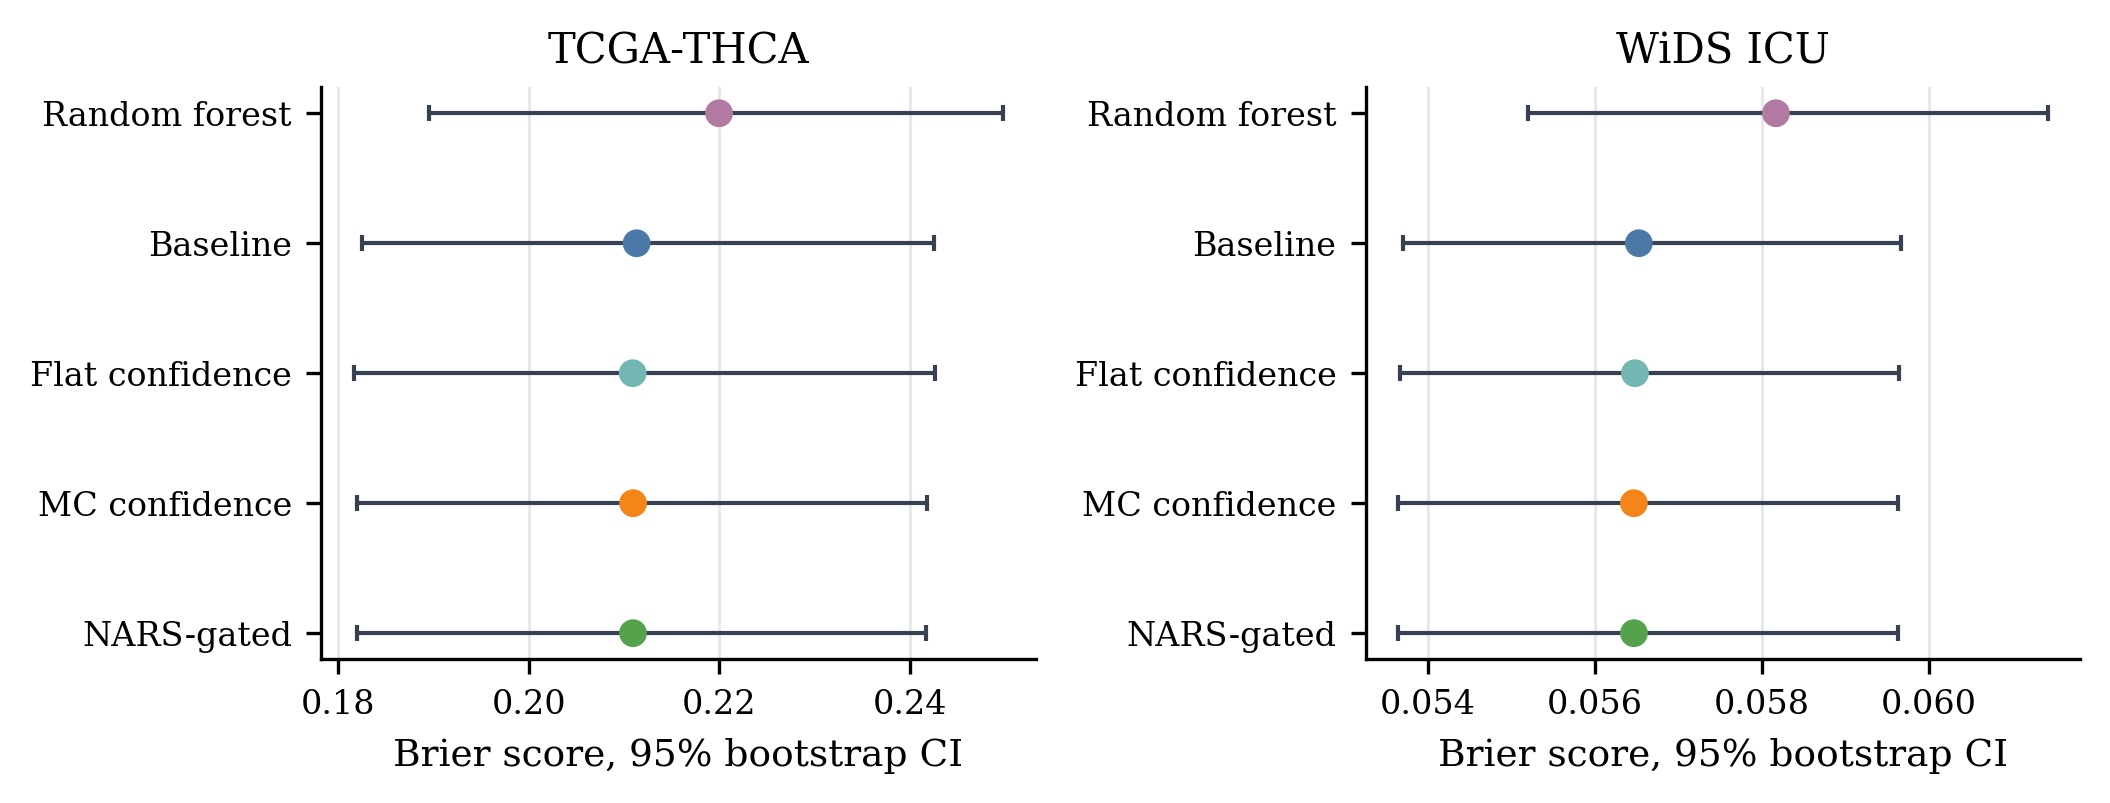
\includegraphics[width=\linewidth]{figures/figure-2-performance-ci.png}
\caption{Held-out Brier scores with 95\% bootstrap confidence intervals. Lower values are better. The transformer variants are close, so small point-estimate differences should be interpreted as descriptive unless corroborated by additional comparisons.}
\label{fig:performance_ci}
\end{figure}

The symbolic pathway operated at scale: ICU rules fired on 8,551 of 13,757 held-out stays, with 13,031 feature-level revisions. The per-rule counts were 1,936 for lactate, 5,338 for hypotension, 3,443 for age, and 2,314 for creatinine. Every fired rule mapped to a feature, produced a finite trace, and changed confidence and attention. The corresponding TCGA rates were also 100\% across 79 events in 42 of 69 cases. Independently recomputed revision and normalized-gating residuals were zero for both datasets.

\IfFileExists{figures/generated_auditability_table.tex}{
% Auto-generated by src.paper_figures.generate_paper_figures.
\begin{table}[t]
\caption{Operational auditability on held-out cases. Completeness and residuals test whether traces faithfully expose the implemented arithmetic; they do not measure clinician usability or rule validity.}
\label{tab:auditability}
\centering
\scriptsize
\setlength{\tabcolsep}{3pt}
\begin{tabular}{@{}lrrrrrr@{}}
\toprule
Data & Cases covered & Events & Complete & $c$ changed & Flips & Max residual \\ 
\midrule
TCGA-THCA & 42/69 (60.9\%) & 79 & 100.0\% & 100.0\% & 0 & 0.0e+00 \\
WiDS ICU & 8,551/13,757 (62.2\%) & 13,031 & 100.0\% & 100.0\% & 10 & 0.0e+00 \\
\bottomrule
\end{tabular}
\end{table}

Table~\ref{tab:auditability} evaluates operational auditability over every held-out rule event. Mapping coverage asks whether a fired proposition reached a model feature; completeness asks whether all values needed for inspection are finite; and residuals independently recompute NAL revision and normalized gating. Among triggered cases, the mean absolute baseline-to-NARS probability change was 0.00205 on TCGA and 0.00214 on WiDS, with maxima of 0.00600 and 0.03102. No triggered TCGA case crossed the 0.5 threshold, while 10 triggered WiDS cases did. These are system-fidelity checks, not evidence that clinicians find the traces useful or that a changed decision is clinically correct.
}{}

\subsection{Case-Level Rule Trace}

The refreshed prediction export provides a concrete held-out example. For WiDS encounter 8205 (target 0), the ungated probability was 0.5006, flat-confidence gating produced 0.4995, MC-confidence-only gating produced 0.4961, and NARS-gated routing produced 0.4968. Three rules fired: hypotension, lactate, and creatinine. Their attention weights changed from 0.2564 to 0.2526, 0.0231 to 0.0248, and 0.0347 to 0.0372, respectively. The trace therefore exposes a real threshold change and the rule-level arithmetic, but it also shows why attribution requires controls: MC-confidence-only had already crossed the threshold before symbolic revision. Across the complete WiDS export, MC-confidence-only and NARS-gated produced no different threshold decisions. This is operational auditability, not clinical validation.

\subsection{Calibration Interpretation}

The WiDS calibration results support a two-part interpretation. Relative to the ungated transformer, NARS-gated routing lowers Brier by 0.0000587 with a paired 95\% interval of [0.0000249, 0.0000911], and lowers ECE by 0.00120 with an interval of [0.0000282, 0.00202]. Both intervals exclude zero. Relative to flat-confidence and MC-confidence-only gating, however, the paired Brier and ECE intervals include zero; MC-confidence-only also has the slightly better Brier and ECE point estimates. Thus the run supports a small benefit from confidence gating, but does not identify symbolic revision as its cause.

That restraint keeps the contribution aligned with what the experiment actually supports. Dynamic evidential routing should not be described as a universal calibration booster. The supported claim is that a symbolic evidential channel can be made active, traceable, and compatible with competitive calibrated prediction on a large high-missingness ICU benchmark.

\section{Discussion and Ablation}
\label{sec:analysis}

The flat-confidence and MC-confidence-only controls are essential for interpreting the result. If NARS-gated attention were compared only with the baseline transformer, its paired Brier and ECE differences could be over-interpreted as a symbolic reasoning effect. The controls show a more precise picture: those differences are not separated from confidence gating before symbolic revision is added. The NARS rule path is therefore best interpreted as an instrumentation layer whose demonstrated value is auditability, modifiability, and compatibility with symbolic intervention, not yet a statistically isolated source of within-family calibration change.

\IfFileExists{figures/figure-3-ablation.png}{
Figure~\ref{fig:ablation} reports the gamma sweeps and decision curves rather than treating them as future experiments. Across $\gamma\in\{0.25,0.5,1,2,4\}$, Brier deltas remain small. On WiDS, stronger gating monotonically lowers the Brier point estimate relative to baseline, reaching a delta of $-6.85\times10^{-5}$ at $\gamma=4$, while AUC deltas remain slightly negative. On TCGA, all five Brier deltas are negative but the small split gives no separated superiority regime. Decision curves likewise show closely overlapping transformer variants with modest threshold-dependent differences.
\begin{figure}[t]
\centering
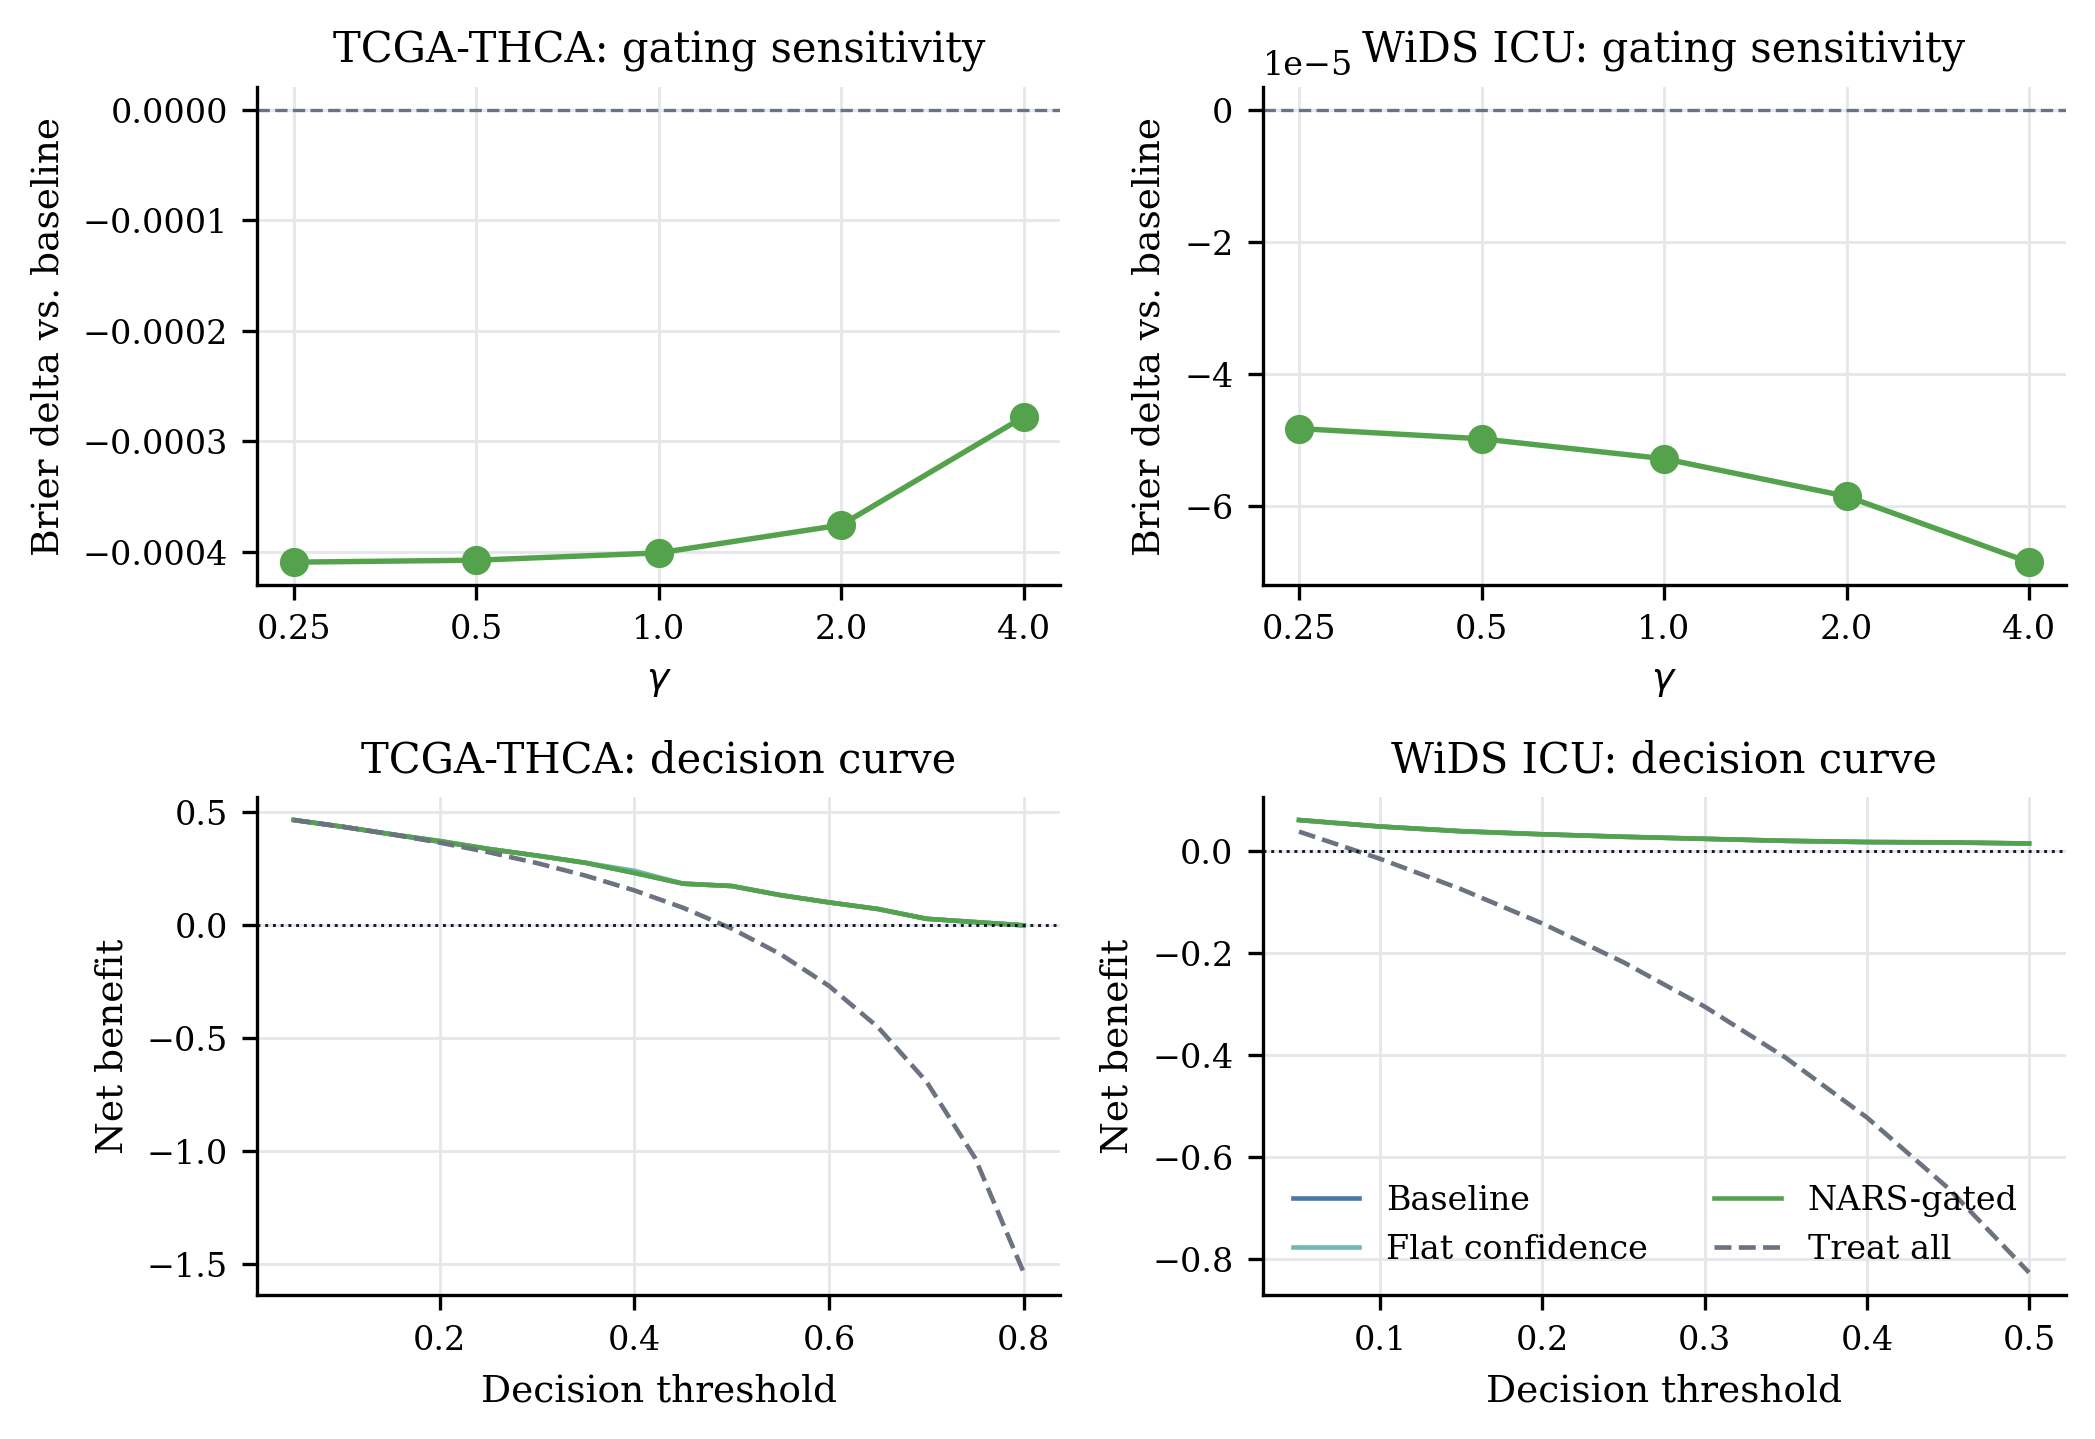
\includegraphics[width=\linewidth]{figures/figure-3-ablation.png}
\caption{Reported ablations. Top: NARS-gated Brier change relative to the ungated transformer across $\gamma$ (negative is lower). Bottom: held-out decision curves over informative threshold ranges. These descriptive curves do not establish clinical utility.}
\label{fig:ablation}
\end{figure}}{}

\subsection{Failure Modes}

The interface can fail in three main ways. First, the neural uncertainty estimate can be wrong. If MC dropout underestimates epistemic uncertainty under shift, the initializer in Eq.~\eqref{eq:neural_to_nars} will assign confidence that is too high. Second, proposition extraction can misalign encoded features with clinical concepts. A one-hot category, imputed value, or missingness indicator may not correspond cleanly to the symbolic condition. Third, the rule truth values can be weak, conflicting, or clinically disputed.

These are general risks whenever learned uncertainty is coupled to external rules, not failures caused by the baseline or control variants. Dynamic evidential routing makes them inspectable: a bad rule leaves a trace, a misfired proposition can be counted, and the gate can be ablated. The interface is not a clinical safety mechanism by itself.

\subsection{What Would Count as Stronger Evidence?}

Stronger evidence would require at least three additions. First, the rule base should be curated independently of the evaluation split, preferably with multiple clinicians or domain experts assigning truth values and resolving disagreement. Second, external validation should be performed without retuning the preprocessing, thresholds, or rule definitions. Third, uncertainty estimators should be compared directly, including MC dropout, deep ensembles, and possibly conformal or distribution-shift-aware variants.

The most informative future ablation would freeze the trained transformer and evaluate four inference modes on multiple external cohorts: baseline attention, flat-confidence attention, MC-confidence attention, and NARS-revised attention. Symbolic revision would be isolated only if NARS-revised attention separates from the first three modes on calibration or decision utility with intervals that exclude zero.

\subsection{Clinical Audit Scenario}

A practical use case for the trace interface is review of cases near a decision threshold. Suppose the model predicts a risk close to an escalation threshold and the final probability changes after a hypotension rule fires. The exported trace can show the original neural truth value, the rule's symbolic truth value, the revised confidence, and the resulting attention gain. A clinician or reviewer can then ask whether the rule condition was extracted correctly and whether the assigned symbolic truth value is appropriate for that clinical context.

This is different from asking whether an attention heat map looks plausible. The trace records a concrete intervention in the computation. If the rule is considered inappropriate, it can be edited or disabled and the same case can be rerun. That workflow is modest, but it is a realistic step toward human-in-the-loop neurosymbolic clinical systems.

\subsection{Deployment Boundary}

The current system is not a clinical decision device. It has no external validation, prospective monitoring, independently curated rule ontology, or clinician-facing user study. Its appropriate status is a methods prototype for studying how neural uncertainty and symbolic evidence can share a truth-value interface.

The deployment boundary also shapes how the metrics should be read. Competitive AUC and calibration are necessary but insufficient. Depending on intended use and jurisdiction, clinical decision-support software may remain subject to medical-device oversight; current U.S. guidance distinguishes non-device CDS from functions that remain devices \citep{fda2026}. A deployment would need locked preprocessing, external validation, shift monitoring, rule governance, human-factors evidence, and clinician override. Inspectable traces could contribute evidence for review, but do not themselves satisfy regulatory or clinical requirements.

\section{Limitations}
\label{sec:limitations}

The current evidence is a methods evaluation, not a clinical validation study. TCGA has only 69 held-out cases, so tiny AUC and calibration differences are not reliable. WiDS is much larger, but all experiments use an internal split rather than an external temporal or institutional cohort. The rule bases are prototype probes; deployment would require independently curated rules, sensitivity analysis, and clinician review.

The neural-to-NAL initializer depends on MC-dropout variance, which can be miscalibrated under shift. The method would over-trust a weak prediction if the uncertainty estimator underestimates epistemic uncertainty. Future runs should compare MC dropout with ensembles and should test shifted cohorts.

Finally, the repository implements NAL truth-value functions and feature-level rule revision, but not the complete NARS architecture. It does not maintain concept priority dynamics, task scheduling, or explicit evidential-base records. The claims should therefore be read as interface-level claims about truth-value-guided fusion and attention control.

\section{Conclusion}
\label{sec:conclusion}

Dynamic evidential routing provides an auditable inference-time interface for uncertainty-aware clinical prediction under missingness while preserving comparable held-out behavior. Across TCGA-THCA and WiDS ICU, explicit rules revise NAL-style confidence, alter normalized attention, and export complete arithmetic traces; the ICU experiment demonstrates that path at scale. On WiDS, paired comparisons support small Brier and ECE improvements over the ungated transformer, while flat-confidence and MC-confidence-only controls prevent attributing those improvements specifically to symbolic revision. Future work should test clinician-curated and conflict-aware rule bases, stronger uncertainty estimators, external cohorts, and human evaluation of whether the traces support real review decisions.

\section*{Ethics, Data, and Code Availability}

This work uses public, de-identified benchmark data and did not collect new patient data. Code and generated artifacts are available at \url{https://github.com/arjuncodess/ngta}. Large language models assisted with drafting, mathematical formulation, and code generation; the author independently checked the derivations, implementation, references, and reported results and takes full responsibility for the work.

\acks{The author thanks Pei Wang for feedback on the distinction between statistical variance and NAL evidence amount, and on the manuscript's deduction-confidence formulation. The author also thanks Prof. Leilani H. Gilpin for detailed feedback on the central neurosymbolic-systems framing, NAL/NARS boundary, pipeline and audit-trace presentation, rule-base discussion, references, and calibration claims. Finally, the author thanks the NeSy 2026 reviewers for their careful reviews and constructive feedback.}

\bibliography{references}

\end{document}
